\documentclass[review,nonacm,acmsmall]{acmart}

\setcopyright{none}
\citestyle{acmauthoryear}

\usepackage{booktabs}
\usepackage{graphicx}
\usepackage{float}
\usepackage{listings}
\usepackage{xcolor}
\usepackage{tikz}
\usetikzlibrary{positioning,arrows.meta,fit}
\usepackage{cleveref}
\usepackage[T1]{fontenc}
\usepackage[utf8]{inputenc}

\crefname{lstlisting}{listing}{listings}
\Crefname{lstlisting}{Listing}{Listings}

% Placeholder for a missing number, citation or text. None may remain at submission.
\providecommand{\todo}[1]{\textcolor{red}{[TODO: #1]}}

% Numbers from experiments/ (never typed by hand).
% Generated by experiments/paper_numbers.py -- do not edit by hand.
\newcommand{\NumMethods}{160}
\newcommand{\NumMethodsOrig}{145}
\newcommand{\NumGuardsMethods}{15}
\newcommand{\NumCases}{297}
\newcommand{\NumGuardsCases}{31}
\newcommand{\NumSites}{408}
\newcommand{\NumSitesNoGuards}{344}
\newcommand{\NumSiteMethods}{100}
\newcommand{\NumUncertain}{368}
\newcommand{\NumNoState}{19}
\newcommand{\NumSettled}{21}
\newcommand{\NumStrict}{215}
\newcommand{\NumStrictMethods}{49}
\newcommand{\NumRuleInvert}{82}
\newcommand{\NumRuleSwap}{178}
\newcommand{\NumRuleStrict}{87}
\newcommand{\NumRuleSplit}{61}
\newcommand{\UncertainPercent}{90}
\newcommand{\NumCompile}{408}
\newcommand{\NumValid}{408}
\newcommand{\InputsMin}{1}
\newcommand{\InputsMax}{128}
\newcommand{\NumCondBoth}{182}
\newcommand{\NumCondOne}{1}
\newcommand{\NumCondUnknown}{225}
\newcommand{\NumOneInput}{7}
\newcommand{\NumMutants}{260}
\newcommand{\NumMutantsEquivalent}{31}
\newcommand{\NumMutantsNonEquivalent}{229}
\newcommand{\NumMutantsKilled}{227}
\newcommand{\NumMutantsSurvived}{2}
\newcommand{\NumNarrowBeatsInterval}{11}
\newcommand{\NumIntervalBeatsNarrow}{3}
\newcommand{\NumNarrowIntervalIncomparable}{0}
\newcommand{\NumNarrowBeatsIntervalOrig}{9}
\newcommand{\NumIntervalBeatsNarrowOrig}{1}
\newcommand{\NumNarrowIntervalIncomparableOrig}{0}
\newcommand{\NumSeeds}{10}
\newcommand{\NumInconsistentVariants}{4}
\newcommand{\NumInconsistentPairs}{6}
\newcommand{\Eligible}{408}
\newcommand{\Pool}{5}
\newcommand{\PoolSign}{2}
\newcommand{\PoolSignNarrow}{3}
\newcommand{\PoolInterval}{0}
\newcommand{\BudgetHalf}{204}
\newcommand{\MeanRandomHalf}{3.1}
\newcommand{\MeanSyntaxHalf}{3.6}
\newcommand{\MeanGuidedHalf}{0.3}
\newcommand{\MeanGuidedStrictHalf}{0.0}
\newcommand{\MeanSettledHalf}{5.0}
\newcommand{\PGuidedRandomHalf}{0.002}
\newcommand{\AGuidedRandomHalf}{0.10}
\newcommand{\PGuidedSyntaxHalf}{$<0.001$}
\newcommand{\AGuidedSyntaxHalf}{0.00}
\newcommand{\PGuidedStrictRandomHalf}{$<0.001$}
\newcommand{\AGuidedStrictRandomHalf}{0.05}
\newcommand{\PGuidedStrictSyntaxHalf}{$<0.001$}
\newcommand{\AGuidedStrictSyntaxHalf}{0.00}
\newcommand{\PSettledRandomHalf}{0.006}
\newcommand{\ASettledRandomHalf}{0.80}
\newcommand{\BudgetQuarter}{102}
\newcommand{\MeanRandomQuarter}{2.4}
\newcommand{\MeanSyntaxQuarter}{0.9}
\newcommand{\MeanGuidedQuarter}{0.1}
\newcommand{\MeanGuidedStrictQuarter}{0.0}
\newcommand{\MeanSettledQuarter}{5.0}
\newcommand{\PGuidedRandomQuarter}{$<0.001$}
\newcommand{\AGuidedRandomQuarter}{0.07}
\newcommand{\PGuidedSyntaxQuarter}{$<0.001$}
\newcommand{\AGuidedSyntaxQuarter}{0.10}
\newcommand{\PGuidedStrictRandomQuarter}{$<0.001$}
\newcommand{\AGuidedStrictRandomQuarter}{0.05}
\newcommand{\PGuidedStrictSyntaxQuarter}{$<0.001$}
\newcommand{\AGuidedStrictSyntaxQuarter}{0.05}
\newcommand{\PSettledRandomQuarter}{$<0.001$}
\newcommand{\ASettledRandomQuarter}{0.95}
\newcommand{\EligibleNoGuards}{344}
\newcommand{\PoolNoGuards}{4}
\newcommand{\PoolSignNoGuards}{2}
\newcommand{\PoolSignNarrowNoGuards}{2}
\newcommand{\PoolIntervalNoGuards}{0}
\newcommand{\BudgetHalfNoGuards}{172}
\newcommand{\MeanRandomHalfNoGuards}{2.2}
\newcommand{\MeanSyntaxHalfNoGuards}{2.6}
\newcommand{\MeanGuidedHalfNoGuards}{0.0}
\newcommand{\MeanGuidedStrictHalfNoGuards}{0.0}
\newcommand{\MeanSettledHalfNoGuards}{4.0}
\newcommand{\PGuidedRandomHalfNoGuards}{0.002}
\newcommand{\AGuidedRandomHalfNoGuards}{0.15}
\newcommand{\PGuidedSyntaxHalfNoGuards}{$<0.001$}
\newcommand{\AGuidedSyntaxHalfNoGuards}{0.00}
\newcommand{\PGuidedStrictRandomHalfNoGuards}{0.002}
\newcommand{\AGuidedStrictRandomHalfNoGuards}{0.15}
\newcommand{\PGuidedStrictSyntaxHalfNoGuards}{$<0.001$}
\newcommand{\AGuidedStrictSyntaxHalfNoGuards}{0.00}
\newcommand{\PSettledRandomHalfNoGuards}{0.006}
\newcommand{\ASettledRandomHalfNoGuards}{0.80}
\newcommand{\BudgetQuarterNoGuards}{86}
\newcommand{\MeanRandomQuarterNoGuards}{1.8}
\newcommand{\MeanSyntaxQuarterNoGuards}{0.0}
\newcommand{\MeanGuidedQuarterNoGuards}{0.0}
\newcommand{\MeanGuidedStrictQuarterNoGuards}{0.0}
\newcommand{\MeanSettledQuarterNoGuards}{4.0}
\newcommand{\PGuidedRandomQuarterNoGuards}{0.002}
\newcommand{\AGuidedRandomQuarterNoGuards}{0.15}
\newcommand{\PGuidedSyntaxQuarterNoGuards}{--}
\newcommand{\AGuidedSyntaxQuarterNoGuards}{0.50}
\newcommand{\PGuidedStrictRandomQuarterNoGuards}{0.002}
\newcommand{\AGuidedStrictRandomQuarterNoGuards}{0.15}
\newcommand{\PGuidedStrictSyntaxQuarterNoGuards}{--}
\newcommand{\AGuidedStrictSyntaxQuarterNoGuards}{0.50}
\newcommand{\PSettledRandomQuarterNoGuards}{$<0.001$}
\newcommand{\ASettledRandomQuarterNoGuards}{0.90}
\newcommand{\CostTotal}{234}
\newcommand{\CostExport}{0.3}
\newcommand{\CostSites}{0.1}
\newcommand{\CostSelection}{0.1}
\newcommand{\CostValidation}{231.7}
\newcommand{\CostAnalysis}{1.8}


\lstset{
    language=Java,
    basicstyle=\ttfamily\footnotesize,
    keywordstyle=\color{blue!65!black},
    columns=fullflexible,
    keepspaces=true,
    showstringspaces=false,
    breaklines=true,
    frame=single
}

\title{Analysis-Guided Metamorphic Testing of Java Static Analyzers}

\author{Hasan Ahmed (s262722)}
\affiliation{%
  \institution{Technical University of Denmark}
  \city{Kongens Lyngby}
  \country{Denmark}}

\begin{document}

% Abstract (~0.25 p). Problem -> key observation (a rewrite changes a result only
% where precision depends on the form of the code) -> technique -> setup (three
% analyzers, three strategies, ten seeds) -> main result, numbers from experiments/.
\begin{abstract}
\todo{abstract: written last}
\end{abstract}


\maketitle

% 1 Introduction (~1.4 p). Terms are only introduced here; Section 4 defines them.
\section{Introduction}
\label{sec:intro}

\paragraph{Context}
A static analyzer predicts which runtime errors a program can reach without
running it on every input. Its precision can depend on how the program is
written. The two Java methods below are equivalent: for every \texttt{int}
input they return the same value and never divide by zero.

\noindent
\begin{minipage}[t]{0.47\linewidth}
\begin{lstlisting}
int f(int x) {
  if (x > 0)
    return 100 / x;
  return 0;
}
\end{lstlisting}
\end{minipage}
\hfill
\begin{minipage}[t]{0.47\linewidth}
\begin{lstlisting}
int f(int x) {
  if (x <= 0)
    return 0;
  return 100 / x;
}
\end{lstlisting}
\end{minipage}

\noindent
An imprecise analyzer may nevertheless warn about a division by zero in one of
them and not in the other. Such a discrepancy need not be unsound; it shows that
the analyzer's over-approximation depends on the form of the code, which
developers experience as warnings that appear or disappear after a harmless
refactoring; real Java analyzers do change their warnings under such
transformations~\citep{zhang2023statfier}. Rewriting a program in a semantics-preserving way and comparing
the analyzer's answers is a metamorphic test that needs no ground truth.

\paragraph{Gap}
Most techniques for testing static analyzers compare against a reference:
other analyzers, concrete execution, or a
solver~\citep{klinger2019,cuoq2012,taneja2020}. Metamorphic testing needs
none~\citep{chen2018}, and equivalence-preserving transformations have exposed
compiler bugs~\citep{le2014emi,donaldson2017}, but where to rewrite for an
analyzer that predicts outcomes is open. Statfier~\citep{zhang2023statfier}
transforms code at warning lines, which such an analyzer does not report;
interrogation testing~\citep{kaindlstorfer2024} changes assertions on purpose
instead of preserving behavior. Earlier DTU work renamed identifiers to test an
LLM and Infer~\citep{chand2024}, which leaves the bytecode instructions that
our analyzers read unchanged, and used abstract states to guide a fuzzer on
JPAMB~\citep{domingues2025}, but an analyzer's prediction for a method does not
depend on runtime inputs. No existing technique therefore says where to place
a behavior-preserving rewrite for such analyzers (\cref{sec:related}).

\paragraph{Innovation}
We ask: \emph{can the abstract state computed by a fixed interval analysis select
semantics-preserving rewrite sites that reveal inconsistencies in a static
analyzer more efficiently than random or syntax-based selection?} The
intuition is that a rewrite can only change an answer where the analyzer's
precision depends on the form of the code. Where a fixed interval analysis,
the \emph{guide}, already decides a branch, a rewritten condition should be
decided the same way; where the guide is uncertain, the analyzer may be too.
We therefore mark sites as \emph{uncertain} from the guide's abstract state and
spend a fixed rewrite budget on them first. The guide's abstract states, not an
analyzer's reported warnings, mark the sites, so the approach applies to
analyzers that predict sets of outcomes rather than lists of warnings.

\paragraph{Evaluation}
We test three abstract interpreters for JPAMB that differ only in their integer
domain and in whether they refine at branches, on \NumMethods{} methods with
\NumSites{} eligible sites, and compare guided selection with random and
syntax-based selection under the same budget over \NumSeeds{} seeds. The
hypothesis does not hold. All \NumValid{} variants are valid, but rewriting
every site exposes only \Pool{} distinct inconsistencies. At a budget of half the sites, guided selection finds
\MeanGuidedHalf{} distinct inconsistencies per run (summed over the three
analyzers), against \MeanRandomHalf{} for random selection
(\PGuidedRandomHalf), and it also loses at a quarter of the sites and without
the cases we added. The reason is a mismatch between guide and analyzers:
\PoolFromSettledOnly{} of the \Pool{} inconsistencies occur at sites the guide
settles, where the rewrite replaces a constant the sign domain abstracts
exactly ($0$) by one it does not ($1$).

\paragraph{Contributions}
\begin{enumerate}
  \item A definition of uncertain sites from a guide's abstract states
    (\cref{sec:sites}).
  \item Four rewrite rules for \texttt{int} conditions with preconditions, and
    test-based validation checked with wrong rewrites
    (\cref{sec:rules,sec:validation,sec:rq3}).
  \item A controlled comparison of guided, random and syntax-based selection
    under one budget on three analyzers, with a negative result and its
    explanation: a guide should model how the analyzer under test abstracts
    constants, not only where the program is undecided
    (\cref{sec:rq1,sec:findings}).
  \item \NumGuardsMethods{} new JPAMB methods with \NumGuardsCases{} annotated
    cases on integer guards (\cref{sec:setup}).
\end{enumerate}

% 2 Background (~1.0 p). The analyzers are the subjects of the study, not its
% contribution, so they are kept apart from the technique.
\section{Background}
\label{sec:background}

\subsection{JPAMB and Outcome Predictions}
\label{sec:jpamb}
JPAMB (Java Program Analysis Micro Benchmarks)~\citep{kalhauge2026jpamb} is a suite
of small static Java methods, each annotated with test cases that state which
outcome an input produces, for example that input \texttt{(0)} leads to a
division by zero. An analyzer receives a method identifier and the bytecode,
and answers, for each of six outcomes, whether some input reaches it: normal
termination (\texttt{ok}), divide by zero, assertion error, out of bounds,
null pointer, and non-termination (\texttt{*}). We call the outcomes it
answers \emph{yes} to its \emph{outcome set} for the method. An analyzer is
sound for a method if the outcome set contains every outcome some input
reaches, and precise if it contains no other. JPAMB scores the answers against
the outcomes of the annotated cases.

\subsection{Metamorphic Testing}
\label{sec:mt}
Metamorphic testing replaces a missing oracle by a \emph{metamorphic
relation} between the outputs for related inputs~\citep{chen2018}. Our system
under test is an analyzer and its inputs are methods. The relation is: two
methods with the same behavior on every input get the same outcome set. A
sound and fully precise analyzer satisfies it trivially, because both outcome
sets equal the true one. A sound but imprecise analyzer over-approximates, and
how much it over-approximates may depend on how the method is written. A
violation, an inconsistency, shows that one of the two outcome sets is
imprecise or, if a reachable outcome is missing, unsound (\cref{sec:inconsistency} defines how we count them). The relation is a
robustness property rather than a correctness requirement.

\subsection{The Three Analyzers Under Test}
\label{sec:analyzers}
The three analyzers are abstract interpreters~\citep{cousot1977} over JPAMB
bytecode. They share one implementation and differ only in the abstract domain
for integers and in whether they refine values at conditional jumps
(\cref{tab:analyzers}). Each computes a fixpoint over the method's
control-flow graph with a worklist. The outcome set collects what the reachable
abstract states can produce: \texttt{ok} at a return; divide by zero at a
\texttt{/} or \texttt{\%} whose divisor may be 0; null pointer at an array
access whose reference may be null, and out of bounds at every array access
whose reference may be non-null, because no domain tracks array lengths;
assertion error at a \texttt{throw}; and \texttt{*} at every reachable
backward jump, so there is no termination analysis. The analysis is
intraprocedural: a call is not analyzed, may raise an assertion error, and
returns an unknown value. References and booleans share the integer domain
(null is 0).

\begin{table}[t]
\caption{The three analyzers under test.}
\label{tab:analyzers}
\small
\begin{tabular}{@{}llll@{}}
\toprule
Analyzer & Domain & Refinement & Widening \\
\midrule
\texttt{static-sign} & subsets of $\{-,0,+\}$ & no & join (finite) \\
\texttt{static-sign-narrow} & subsets of $\{-,0,+\}$ & yes & join (finite) \\
\texttt{static-interval} & intervals $[l,h]$ of 32-bit ints & yes & at loop heads \\
\bottomrule
\end{tabular}
\end{table}

\paragraph{Domains}
Both domains abstract sets of 32-bit integers ordered by inclusion, and both
form Galois connections with them: for signs,
$\alpha(V)=\{\mathrm{sign}(v) \mid v\in V\}$ and
$\gamma(S)=\{v \mid \mathrm{sign}(v)\in S\}$; for intervals,
$\alpha(V)=[\min V,\max V]$ and $\gamma([l,h])=\{v \mid l\le v\le h\}$. We
write $\pm\infty$ for a bound at the 32-bit limit. For \texttt{+}, \texttt{-},
\texttt{*} and \texttt{/}, interval arithmetic computes the hull of the
results at the bounds, and a result that leaves the 32-bit range, where Java
wraps around, becomes $[-\infty,\infty]$; \texttt{\%} uses $|a \% b| < |b|$,
and other operators give $[-\infty,\infty]$. The sign domain ignores
wrap-around, so its predictions are unsound when an operation overflows.

\paragraph{Refinement at branches}
At a conditional jump such as \texttt{if (x > 0)}, an analyzer with refinement
intersects the abstract value of each compared local variable with the values
that make the condition true on one edge and false on the other; a compared
expression such as \texttt{x+1} is not refined. With or without refinement, an
edge is dropped when the comparison cannot have that outcome, but without
refinement its successor receives the unrefined state. This is also called
narrowing at branches, hence the name \texttt{static-sign-narrow}; it is not
the narrowing operator that recovers precision after
widening~\citep{moller2018spa}, which none of the analyzers uses.

\paragraph{Widening}
Every cycle in the control-flow graph contains an edge to an equal or smaller
instruction offset, and the analyzer widens at its target. States at a node
only grow, and at a widening point every strict increase of a bound sets it to
$\pm\infty$, so each widening point changes finitely often and the iteration
terminates. For signs, widening is the join, which suffices because the
lattice is finite; for intervals, ascending chains have length about $2^{33}$,
so iteration without widening could take that many steps.

\paragraph{Neither domain is uniformly more precise}
An interval has no holes: refining $[-\infty,\infty]$ with \texttt{x != 0}
leaves $[-\infty,\infty]$, since \texttt{!=} removes a constant only at an
endpoint (e.g.\ $[0,h]$ becomes $[1,h]$), while \texttt{static-sign-narrow}
obtains $\{-,+\}$ and proves a later \texttt{1 / x} safe. Conversely,
\texttt{static-interval} proves \texttt{if (n > 100) \{ if (n < 50) ... \}}
infeasible, which signs cannot. Of the \NumMethods{} benchmark methods,
\texttt{static-sign-narrow} predicts a strictly smaller outcome set than
\texttt{static-interval} on \NumNarrowBeatsInterval{} and a strictly larger one
on \NumIntervalBeatsNarrow{}, so the analyzers differ in precision for reasons
unrelated to where a rewrite is placed.

% 3 Overview (~1.0 p). One worked example end to end, taken from real pipeline
% output (after step 8), and the pipeline figure (PDI).
\section{Overview}
\label{sec:overview}

% Fig. 1: the pipeline (process diagram).
\begin{figure}[t]
\centering
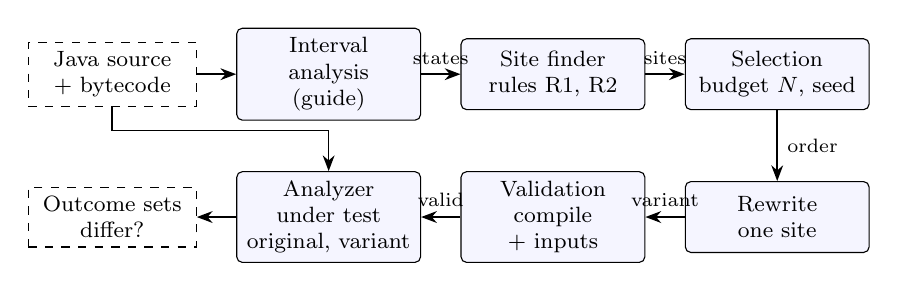
\begin{tikzpicture}[
    font=\footnotesize,
    node distance=4mm and 5mm,
    stage/.style={draw, rounded corners=2pt, align=center, minimum height=9mm,
                  text width=21mm, fill=blue!4},
    data/.style={draw, dashed, align=center, minimum height=7mm, text width=19mm},
    arr/.style={-{Stealth[length=2mm]}, semithick},
  ]
  % row 1: guidance
  \node[data]                        (src)   {Java source\\+ bytecode};
  \node[stage, right=of src]         (guide) {Interval analysis\\(guide)};
  \node[stage, right=of guide]       (find)  {Site finder\\rules R1, R2};
  \node[stage, right=of find]        (sel)   {Selection\\budget $N$, seed};
  % row 2: testing
  \node[stage, below=9mm of sel]     (rw)    {Rewrite\\one site};
  \node[stage, left=of rw]           (val)   {Validation\\compile + inputs};
  \node[stage, left=of val]          (ana)   {Analyzer under test\\original, variant};
  \node[data, left=of ana]           (cmp)   {Outcome sets\\differ?};

  \draw[arr] (src) -- (guide);
  \draw[arr] (guide) -- node[above, font=\scriptsize] {states} (find);
  \draw[arr] (find) -- node[above, font=\scriptsize] {sites} (sel);
  \draw[arr] (sel) -- node[right, font=\scriptsize] {order} (rw);
  \draw[arr] (rw) -- node[above, font=\scriptsize] {variant} (val);
  \draw[arr] (val) -- node[above, font=\scriptsize] {valid} (ana);
  \draw[arr] (ana) -- (cmp);
  \draw[arr] (src.south) -- ++(0,-3mm) -| (ana.north);
\end{tikzpicture}
\caption{The pipeline. An interval analysis computes abstract states that mark
sites as uncertain; a strategy orders the eligible sites, and the first $N$ are
rewritten, one rewrite per variant. Valid variants and their originals are
analyzed by the same analyzer, and an inconsistency is a difference between
the two predicted outcome sets.}
\label{fig:pipeline}
\end{figure}


\todo{worked example: method, interval state at the site, why it is a candidate,
the rewrite, outcome sets of the three analyzers, the inconsistency}

% 4 Analysis-Guided Rewriting (~2.2 p). Defines each term once, in pipeline order.
\section{Analysis-Guided Rewriting}
\label{sec:approach}

\subsection{Consistency and Inconsistencies}
\label{sec:inconsistency}
\todo{the metamorphic relation; the counting unit (D10)}

\subsection{Sites, Uncertain Sites and Candidates}
\label{sec:sites}
\todo{conditions (i) and (ii), computed from the interval state (D14)}

\subsection{Rewrite Rules}
\label{sec:rules}
\todo{R1 branch inversion with swap; R2 equivalent integer comparisons; preconditions;
equivalence arguments; table of rules}

\subsection{Selection Under a Shared Budget}
\label{sec:selection}
\todo{guided, random, syntax-based; one benchmark-wide budget N and a seed (D15)}

\subsection{Validating Variants}
\label{sec:validation}
\todo{compile, synthesized inputs, outcome and return value (D16)}

% 5 Implementation (~0.5 p). Three entry points over one code base (D7), state
% export, mapping bytecode PCs to source sites, tree-sitter site finder, runner.
\section{Implementation}
\label{sec:implementation}
\todo{implementation}

% 6 Evaluation (~2.4 p).
\section{Evaluation}
\label{sec:evaluation}

\subsection{Research Questions}
\label{sec:rqs}
\begin{description}
  \item[RQ1 (effectiveness)] Under the same rewrite budget, does guided
    selection find more distinct inconsistencies than random and
    syntax-based selection?
  \item[RQ2 (cost)] What does each stage of the pipeline cost, and what does
    guidance add?
  \item[RQ3 (validity)] Can the variants be trusted to be equivalent to their
    originals?
\end{description}

\subsection{Subjects and Setup}
\label{sec:setup}
The subjects are \NumMethods{} JPAMB methods: \NumMethodsOrig{} from the
benchmark and \NumGuardsMethods{} methods (\NumGuardsCases{} annotated cases)
in a new class, \texttt{Guards}, written before any RQ1 measurement in five
patterns fixed in advance: guarded division, range checks before array
accesses, branches an analysis can decide, assertions on facts from an earlier
branch, and else-if chains used after the merge. Since the author of the
technique wrote them, every RQ1 result is also reported without them.

There are \NumSites{} eligible sites in \NumSiteMethods{} methods
(\NumSitesNoGuards{} without \texttt{Guards}). \NumUncertain{}
(\UncertainPercent\%) are candidates for \texttt{guided}, \NumStrict{} of them
also strict candidates for \texttt{guided-strict}; \NumSettled{} are settled and \NumNoState{} have no
guide state. The share of candidates is high because many conditions compare
unconstrained parameters, array accesses are always uncertain, and sites on one
line share a flag. The budget is $N=\BudgetHalf$ (50\% of the eligible sites)
or $N=\BudgetQuarter$ (25\%), and $N=\BudgetHalfNoGuards$ or
$N=\BudgetQuarterNoGuards$ without \texttt{Guards}, with \NumSeeds{} seeds per
strategy. The measure is the number of distinct inconsistencies per run,
summed over the three analyzers; the tests use the sum because
\texttt{static-interval} has none, and \cref{tab:rq1} gives the per-analyzer
means. Strategies are compared by a two-sided Mann--Whitney U test (normal
approximation with tie and continuity correction) and the Vargha--Delaney effect size
$\hat{A}_{12}$, the probability that a \emph{run} (one strategy, budget and
seed) of the first strategy finds more
than a run of the second, ties counted half. All runs used one machine:
\Machine.

\subsection{RQ1: Effectiveness}
\label{sec:rq1}
Rewriting \emph{every} eligible site bounds what any strategy can find; we
call these inconsistencies the \emph{pool}. It yields only \Pool{} distinct inconsistencies (\PoolSign{} for
\texttt{static-sign}, \PoolSignNarrow{} for \texttt{static-sign-narrow},
\PoolInterval{} for \texttt{static-interval}), from \NumInconsistentVariants{}
of the \NumValid{} variants, all from R2-strict; without \texttt{Guards}, the
pool is \PoolNoGuards{}. RQ1 therefore asks whether a strategy reaches these
few sites within its budget.

\begin{table}[t]
\caption{RQ1: distinct inconsistencies per run at the 50\% budget, mean
(population standard deviation) over \NumSeeds{} seeds, per analyzer and in total, with
the Mann--Whitney $p$ and $\hat{A}_{12}$ of the total against
\texttt{random}. $^\dagger$Exploratory, defined after the pool was known.}
\label{tab:rq1}
\small
% Generated by experiments/paper_numbers.py -- do not edit by hand.
\begin{tabular}{@{}lrrrrrr@{}}
\toprule
Strategy & \texttt{sign} & \texttt{sign-narrow} & \texttt{interval} & total & $p$ vs.\ random & $\hat{A}_{12}$ \\
\midrule
\multicolumn{7}{@{}l}{\emph{all: 408 sites, $N=204$, pool 5}} \\
\texttt{random} & 1.1 (0.8) & 2.0 (1.0) & 0.0 (0.0) & 3.1 (1.8) &  &  \\
\texttt{syntax} & 1.3 (0.5) & 2.3 (0.5) & 0.0 (0.0) & 3.6 (0.9) &  &  \\
\texttt{guided} & 0.0 (0.0) & 0.3 (0.5) & 0.0 (0.0) & 0.3 (0.5) & 0.002 & 0.10 \\
\texttt{guided-strict} & 0.0 (0.0) & 0.0 (0.0) & 0.0 (0.0) & 0.0 (0.0) & $<0.001$ & 0.05 \\
\texttt{settled}$^\dagger$ & 2.0 (0.0) & 3.0 (0.0) & 0.0 (0.0) & 5.0 (0.0) & 0.006 & 0.80 \\
\midrule
\multicolumn{7}{@{}l}{\emph{without Guards: 344 sites, $N=172$, pool 4}} \\
\texttt{random} & 1.1 (0.8) & 1.1 (0.8) & 0.0 (0.0) & 2.2 (1.7) &  &  \\
\texttt{syntax} & 1.3 (0.5) & 1.3 (0.5) & 0.0 (0.0) & 2.6 (0.9) &  &  \\
\texttt{guided} & 0.0 (0.0) & 0.0 (0.0) & 0.0 (0.0) & 0.0 (0.0) & 0.002 & 0.15 \\
\texttt{guided-strict} & 0.0 (0.0) & 0.0 (0.0) & 0.0 (0.0) & 0.0 (0.0) & 0.002 & 0.15 \\
\texttt{settled}$^\dagger$ & 2.0 (0.0) & 2.0 (0.0) & 0.0 (0.0) & 4.0 (0.0) & 0.006 & 0.80 \\
\bottomrule
\end{tabular}

\end{table}

\Cref{tab:rq1} gives the result. The main strategy,
\texttt{guided}, and its sensitivity variant \texttt{guided-strict} find
\emph{fewer} inconsistencies than \texttt{random} in every setting. At $N=\BudgetHalf$,
\texttt{guided} finds \MeanGuidedHalf{} on average, against \MeanRandomHalf{}
for \texttt{random} (\PGuidedRandomHalf, $\hat{A}_{12}=\AGuidedRandomHalf$) and
\MeanSyntaxHalf{} for \texttt{syntax} (\PGuidedSyntaxHalf); at
$N=\BudgetQuarter$ and without \texttt{Guards} the direction against
\texttt{random} is the same. Of
the \NumPlannedTests{} planned tests that can be computed, the largest $p$ is
\MaxPlannedP{}, below the Bonferroni threshold of \BonferroniAlpha{}; in the
\NumPlannedNoTest{} remaining comparisons, without \texttt{Guards} at
$N=\BudgetQuarterNoGuards$, \texttt{syntax} finds none either. These results
are largely fixed by construction. Because $N$ is smaller than the number of
candidates, \texttt{guided} never reaches a settled site, whatever the seed,
and \NumInconsistentSitesSettled{} of the \NumInconsistentVariants{} sites
that produce an inconsistency are settled; \PoolFromSettledOnly{} of the
\Pool{} distinct inconsistencies come from no uncertain site. The seeds vary
only which of these sites \texttt{random} and \texttt{syntax} reach.

\emph{Answer to RQ1: no. Choosing uncertain sites first finds fewer distinct
inconsistencies than random selection in all four settings, and fewer than
syntax-based selection in three; in the fourth, neither finds any.}

\paragraph{Exploratory: settled sites first}
The opposite order, which we defined only after seeing the pool and therefore
treat as a hypothesis, rewrites the \NumSettled{} settled sites first. Since
\NumSettled{} is below every budget, it contains the whole pool at both
budgets, by construction (\MeanSettledHalf{} in every seed). Whether settled
sites are richer elsewhere would need a new experiment on other analyzers and
programs.

\subsection{RQ2: Cost}
\label{sec:rq2}
One complete run of the pipeline, which reproduces the stored sites,
selections, validation results and outcome sets exactly,
takes \CostTotal{}\,s. Validation dominates with \CostValidation{}\,s:
compiling every variant and running every input on both versions. Computing
the guide's states for all methods takes \CostExport{}\,s, site finding and
selection \CostSites{}\,s and \CostSelection{}\,s, and analyzing every
original and variant with all three analyzers \CostAnalysis{}\,s. Guidance is
thus negligible, and under a time budget every strategy would validate about
the same number of variants, so a time-budget comparison reduces to the
rewrite-budget comparison of RQ1. For the same reason we do not report time to
the first inconsistency, which here is the position of the first of
\NumInconsistentVariants{} sites in each order.

\emph{Answer to RQ2: guidance costs \CostExport{}\,s of \CostTotal{}\,s;
validating the variants dominates the cost.}

\subsection{RQ3: Validity of Variants}
\label{sec:rq3}
All \NumCompile{} variants compile and agree with their originals on every
input, so testing discards \NumDiscarded{}, and \NumBytecodeIdentical{} have
the original's bytecode. To check that the inputs could have exposed a wrong rewrite, we
validated deliberately wrong ones: off-by-one or opposite operators for R2,
and negation without swapping the branches for R1. Of the \NumMutants{}
mutants, \NumMutantsEquivalent{} are equivalent to the original on all inputs
(for example, an off-by-one at a boundary the operand never reaches), each
with a written argument; testing rejects \NumMutantsKilled{} of the other
\NumMutantsNonEquivalent{}. The \NumMutantsSurvived{} survivors need
coordinated values in two or three parameters, which one-at-a-time synthesis
does not produce. For conditions on parameters the method never assigns, we
measured the original condition at entry: for \NumCondBoth{} variants the
inputs make it take both values and for \NumCondOne{} only one; for the other
\NumCondUnknown{} variants this is not measured.

\emph{Answer to RQ3: every variant passed, and the inputs reject all but
\NumMutantsSurvived{} non-equivalent wrong rewrites; the evidence is weaker for
methods with non-integer parameters (\cref{sec:threats}).}

\subsection{What the Inconsistencies Reveal}
\label{sec:findings}
\Cref{tab:inconsistencies} lists the variants that change an outcome set. They
share one cause: the sign domain abstracts the constant $0$ exactly, to
$\{0\}$, but $1$ to $\{+\}$ and $-1$ to $\{-\}$. A value in $\{+\}$ compared
with $\{0\}$ by \texttt{>} is always greater; compared with $\{+\}$ by
\texttt{>=}, it may not be, since the domain cannot tell $1$ from $2$. All
\NumInconsistentSitesCrossZero{} sites are among the \NumStrictCrossZero{}
R2-strict sites whose literal changes to or from $0$.

\begin{table}[t]
\caption{The variants with an inconsistency. Guide: the site's status for the
interval guide. Outcomes: ok, assertion error (AE), divide by zero (DZ),
non-termination ($\ast$).}
\label{tab:inconsistencies}
\small
% Generated by experiments/paper_numbers.py -- do not edit by hand.
\begin{tabular}{@{}lllll@{}}
\toprule
Site & Rewrite & Guide & Analyzers & Original $\to$ variant \\
\midrule
\texttt{Guards:138} & \texttt{x >= 0} $\to$ \texttt{x > -1} & uncertain & \texttt{sign-narrow} & \{ok\} $\to$ \{ok, AE\} \\
\texttt{Guards:139} & \texttt{y > 0} $\to$ \texttt{y >= 1} & settled & \texttt{sign-narrow} & \{ok\} $\to$ \{ok, AE\} \\
\texttt{Loops:19} & \texttt{i > 0} $\to$ \texttt{i >= 1} & settled & \texttt{sign}, \texttt{sign-narrow} & \{$\ast$\} $\to$ \{AE, $\ast$\} \\
\texttt{Loops:27} & \texttt{i > 0} $\to$ \texttt{i >= 1} & settled & \texttt{sign}, \texttt{sign-narrow} & \{$\ast$\} $\to$ \{DZ, $\ast$\} \\
\bottomrule
\end{tabular}

\end{table}

\begin{lstlisting}[float=t,caption={\texttt{Loops.neverAsserts} (left) and
its R2-strict variant (right).},label={lst:loops}]
int i = 1;                        int i = 1;
while (i > 0) {}                  while (i >= 1) {}
assert false;                     assert false;
\end{lstlisting}

In \cref{lst:loops}, both sign analyzers know $i\in\{+\}$. On the left the
loop condition is always true, the assertion is unreachable, and the
prediction is $\{\ast\}$; on the right the condition may be false and an
assertion error is added. \texttt{Loops.neverDivides} is the same with a
division by zero. The interval guide knows $i\in[1,1]$ and decides both
forms, so the site is settled and \texttt{guided} never reaches it within the
budget. \Cref{sec:overview} shows the same effect in a guard.

This explains why the hypothesis behind guidance (\cref{sec:sites}) fails for
these analyzers. The guide represents every constant exactly, the sign domain
only $0$. An inconsistency of this kind needs a comparison that the sign
analyzer decides in one form and not in the other, and such a comparison is
usually decided by the guide in both, so the site is settled. Where the guide is
uncertain, the condition is typically undecided for all three analyzers in
both forms, and the rewrite changes nothing; only
\NumInconsistentSitesUncertain{} of the \NumUncertain{} uncertain sites
produces an inconsistency.

The other rules change no outcome set on JPAMB. On each edge, both domains
refine the two operands of a comparison alike, whichever side they are on and
whichever edge is taken, so swapping operands or inverting a branch gives the
same edge states. For \texttt{static-sign-narrow}, splitting
\texttt{x != y} gives the union of the \texttt{<} and \texttt{>} refinements,
which is the \texttt{!=} refinement, and splitting \texttt{==} gave the same
states as \texttt{==} in every case we checked; for intervals the hull of the two parts equals the
\texttt{!=} refinement, and the sequence of \texttt{<=} and \texttt{>=} the
\texttt{==} refinement. For intervals the fixpoint could still depend on the
order in which a widening point is reached when R1 or R2-split reorders or
adds branches inside a loop, but this does not occur on JPAMB, and R2-strict
is exact for intervals, since $x>c$ and $x\ge c+1$ refine to the same
interval.

% 7 Threats to Validity (~0.4 p). Internal, construct, conclusion, external.
\section{Threats to Validity}
\label{sec:threats}

\paragraph{Internal validity}
A wrong rewrite could create a spurious inconsistency. Each rule has an
equivalence argument and a syntactic precondition, and every variant passed
testing; this is evidence, not a proof, and \cref{sec:rq3} gives its limits
(coordinated values in several parameters, unmeasured conditions). Methods with
non-integer parameters are tested only on their case inputs and simple array
and random-object inputs. For \texttt{static-interval}, the guide and the
analyzer under test coincide, and all three share one implementation, so the
guide knows exactly where they give up; sharing code could only favor
\texttt{guided}, which nevertheless found fewer inconsistencies.

\paragraph{Construct validity}
A distinct inconsistency (\cref{sec:inconsistency}) counts the same change of
outcome set by the same rule in one method once, which may merge different
causes or split one cause over several methods. The per-line uncertainty
flag and the always uncertain array accesses (\cref{sec:setup}) make
\texttt{guided-strict} partly syntactic, and it and \texttt{settled} were
defined after seeing the data, so neither is evidence for the technique. Time
budgets are not reported (\cref{sec:rq2}).

\paragraph{Conclusion validity}
The tests compare \NumSeeds{} runs per strategy whose orders differ only by
the seed over a fixed pool of \Pool{} inconsistencies, with many ties; the
$p$-values describe these runs, and the guided results are largely fixed by
construction (\cref{sec:rq1}).

\paragraph{External validity}
JPAMB consists of micro-benchmarks, the rules cover only \texttt{int}
comparisons, and the three analyzers come from one code base; other analyzers
and programs may contain more inconsistencies. The \texttt{Guards} cases were
written by us, the authors of the technique, but the RQ1 answer holds without
them (\cref{sec:rq1}). Loop
reshaping (\texttt{while} to \texttt{if} with \texttt{do}-\texttt{while}) is
not among the rules, so effects of loop shape on widening are not covered.

% 8 Related Work (~0.75 p). By theme, each ending with how it differs from ours.
% Only citations verified by literature-scout.
\section{Related Work}
\label{sec:related}
\todo{related work}

% 9 Conclusion (~0.25 p). Answer to the RQ, main limitation, future work
% (loop reshaping, reduced product, larger programs).
\section{Conclusion}
\label{sec:conclusion}
\todo{conclusion}


\bibliographystyle{ACM-Reference-Format}
\bibliography{bibfile}

\end{document}
